\section{Vorgehensweise}
Es wurde folgendes Tutorial\cite{tutorial} als Basis für die Aufgabenstellung verwendet:

\href{https://www.sitepoint.com/offline-web-apps-service-workers-pouchdb/}{Create Offline Web Apps Using Service Workers \& PouchDB}

Die fertige Einkaufsliste als Web-App ist hier zu finden: \url{www.github.com/jkopanski2/einkaufsliste}

Als Einstieg in dieses Thema folgt zuerst ein Abschnitt mit allgemeinen Erklärungen.

\section{Offline-First Applikationen}

Sogenannte Offline-First\cite{offlinefirst} Applikationen funktionieren auch, wenn sie keine oder auch nur eine schlechte Internetverbindung haben. Durch das cachen der Seite ist es möglich auf diese auch offline zuzugreifen. Die Daten werden in einer lokalen Datenbank gespeichert, die sich bei einer bestehenden Internetverbindung wieder mit einer anderen Datenbank im Backend synchronisiert. \cite{offlinefirstarticle} Somit kann der Benutzer beispielsweise immernoch Einträge in der Einkaufsliste tätigen, auch wenn er einmal keine Verbindung zum Internet hat.  

\subsection{Mögliche Technologien}
\subsubsection{Couchbase Sync Gateway}
Couchbase hat eine Möglichkeit die mobile Datenbank \textit{Couchbase Lite} mithilfe eines \textit{Couchbase Sync Gateway} mit einem \textit{Couchbase Server} zu synchronisieren. Die Schnittstelle liefert die Daten vom Client an den Server und sorgt somit für eine Sicherung der Daten.

\begin{figure}[!h]
  \begin{center}
    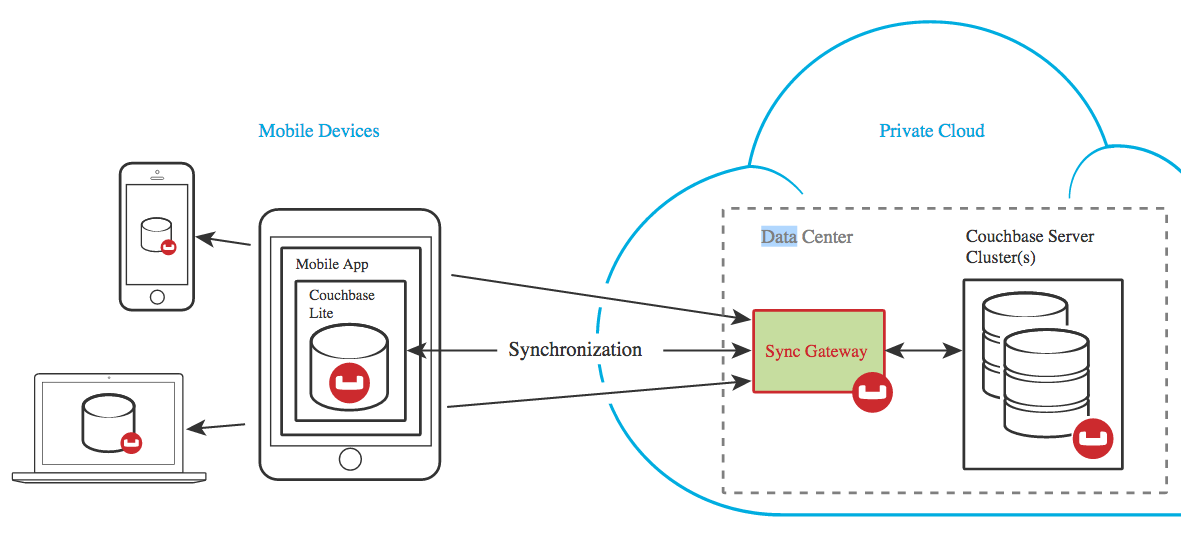
\includegraphics[width=0.7\linewidth]{images/sync_gateway.png}
     \caption{Couchbase Sync Gateway\cite{syncgateway}}
    \label{broker}
  \end{center}
\end{figure}

Hier eine Beispielanwendung, welche die Synchronisation mittels dem \textit{Couchbase Sync Gateway} und die Offline Verfügbarkeit mittels \textit{PouchDB}, welches später erklärt wird, zeigt:
\href{https://www.codementor.io/pmbanugo/using-pouchdb-and-couchbase-in-an-offline-first-application-5pw2sxs6o}{Using PouchDB and Couchbase in an Offline-First Application\cite{syncgatewaytutorial}}

\url{}

\subsection{Firebase Realtime Database}
Mithilfe der Google Plattform Firebase kann man ebenfalls Daten in seiner Web Applikation synchronisieren. Hierfür wird die \textit{Realtime Database}\cite{realtimedb} verwendet, welche die Daten über alle Endgeräte mit der NoSQL Datenbank synchronisiert. Eine Beispielanwendung, welche genau den Anforderungen dieser Übung entspricht, ist hier zu finden: \href{http://softauthor.com/learn-to-build-firebase-crud-app-with-javascript-part01-reading-data/}{Firebase CRUD Web App with Javascript}\cite{firebaseexample} 


\subsection{CouchDB - PouchDB mit Service Worker}
Als lokale Datenbank wird hier die dokementenbasierte Datenbank \textit{PouchDB} verwendet, welche sich mit \textit{CouchDB} synchronisieren lässt. Dies ist problemlos möglich, da \textit{PouchDB} auf dem \textit{CouchDB sync Protkoll}\cite{couchdbsyncprot} basiert.\cite{pouchdbintro} Für das Caching ist ein \textit{Service Worker}\cite{serviceworker} zuständig. Dieser ist zwischen Server und Browser und kann somit steuern, welche Inhalte angezeigt werden sollen. Bei einer mangelnden Internetverbindung liest er die gecachten Daten aus und ermöglicht dem Benutzer somit die Offline Verfügbarkeit.

\begin{figure}[!h]
  \begin{center}
    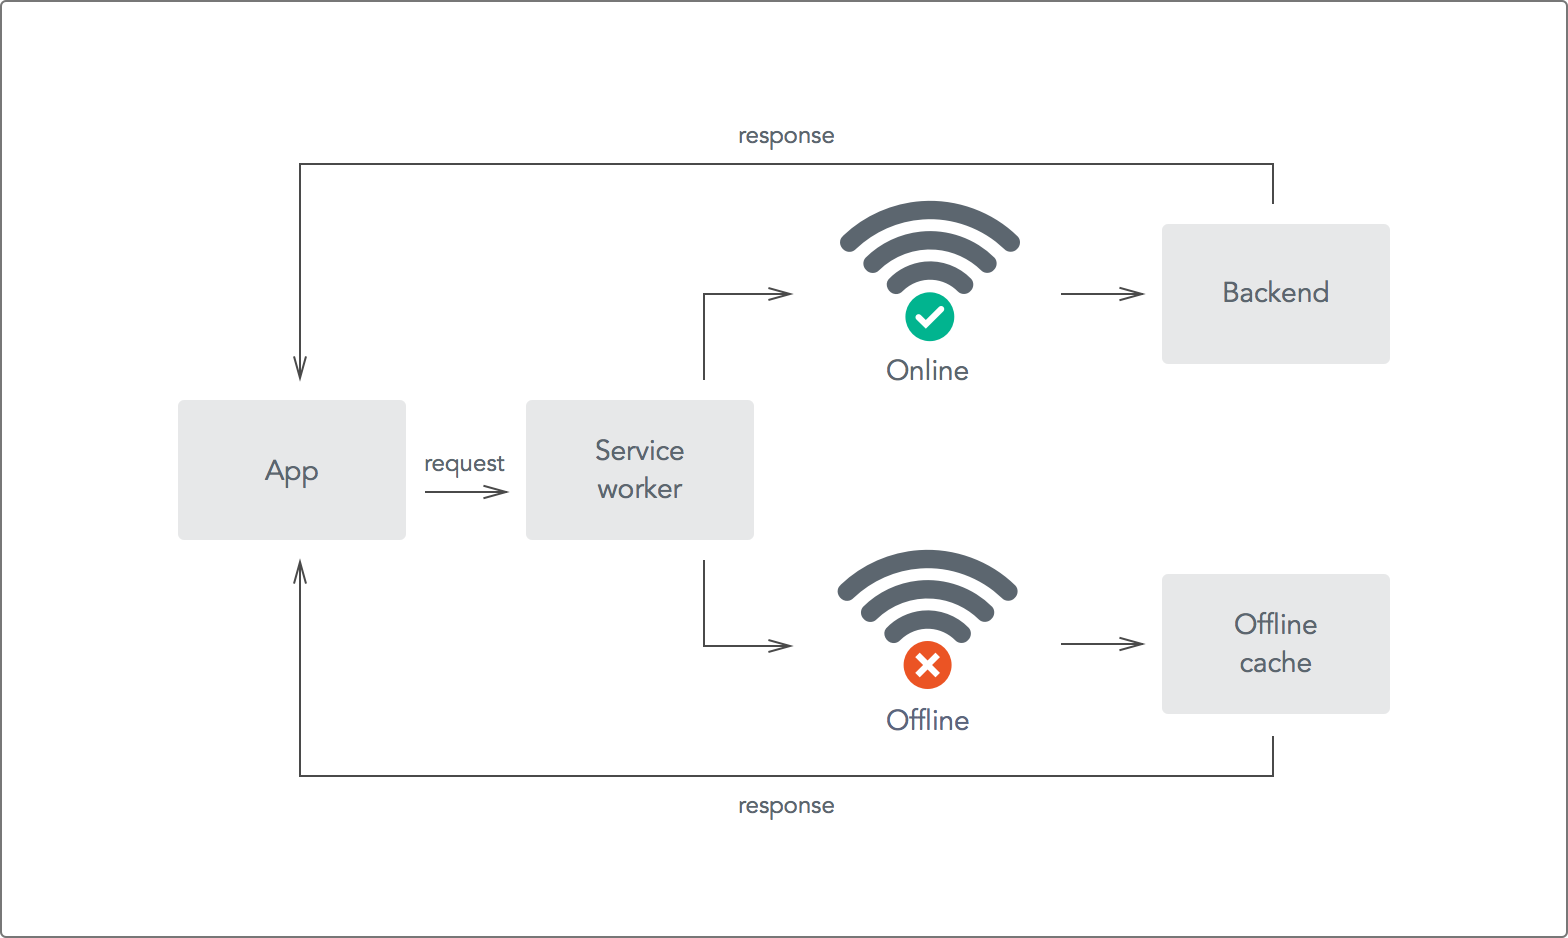
\includegraphics[width=0.7\linewidth]{images/offline-first-diagram.png}
     \caption{Service Worker\cite{serviceworkertutorial}}
    \label{broker}
  \end{center}
\end{figure}

%Coucbase mit Sync Gateway
%Firebase 
%Pouchdb mit Couchdb / Caching mittels Serviceworker


\subsection{Gewählte Technologie}

Durch die fast automatische Replikation der Daten zwischen \textit{PouchDB} und \textit{CouchDB} wurde dieser Ansatz gewählt. In der Hoffnung sich komplexe Konfigurationen, wie es beispielsweise bei \textit{Couchbase} der Fall ist, zu ersparen. Die Google-Lösung mittels Firebase wurde ausgelassen, da man eine \enquote{kleinere} Lösungen ausprobieren wollte.

\section{Implementierung}

\subsection{Service Worker}

Zu Beginn wird überprüft ob der \textit{Service Worker} vom Browser unterstützt wird. Wenn ja, wird die Methode zum Registrieren aufgerufen. In diesem Fall ist es die \textit{service-worker.js}, welche aufgerufen wird:

\begin{lstlisting}[language=JavaScript]
if ('serviceWorker' in navigator) {
    navigator.serviceWorker.register('/service-worker.js', {
        scope: '/'
    }).then(function() {
        // success
    }).catch(function(e) {
        // failed
    });
}

\end{lstlisting}

Danach wird der \textit{Service Worker} installiert. Hierfür muss unter anderem angegeben werden, welche Files gechacht werden sollen.

\begin{lstlisting}[language=JavaScript]
var CACHE_NAME = 'einkaufsliste';

var resourcesToCache = [
  '/',
  '/css/style.css',
  '/js/ext/babel.min.js',
  '/js/ext/pouchdb.min.js',
  '/js/register-service-worker.js',
  '/js/store.js',
  '/js/app.js'
];

self.addEventListener('install', function(event) {
  event.waitUntil(
    // open the app browser cache
    caches.open(CACHE_NAME)
      .then(function(cache) {
        // add all app assets to the cache
        return cache.addAll(resourcesToCache);
      })
  );
});

\end{lstlisting}

Zuletzt wird noch festgelegt, wie auf das fetch-event\cite{fetch} reagiert werden soll, welches bei jedem Request einer Seite ausgelöst wird. 

\begin{lstlisting}[language=JavaScript]
self.addEventListener('fetch', function(event) {
  event.respondWith(
    // try to find corresponding response in the cache
    caches.match(event.request)
      .then(function(response) {
        if (response) {
          // cache hit: return cached result
          return response;
        }

        // not found: fetch resource from the server
        return fetch(event.request);
      })
  );
});
\end{lstlisting}

Der \textit{Service Worker} wird derzeit noch nicht von allen Browsern unterstützt\cite{sworkerusage}, weswegen zusätzlich noch der AppCache\cite{appcache} eingerichtet wird. 

\subsection{PouchDB und CouchDB}

Für die lokale Datenspeicherung ist \textit{PouchDB} zuständig. Die Idee dahinter ist, in der Zeit in der keine Internetverbindung besteht, die Daten lokal zu speichern und bei wiederkommender Verbindung diese dann mit \textit{CouchDB} zu synchronisieren. 

Hierfür wurden benötigte CRUD-Funktionen implementiert:
\begin{lstlisting}[language=JavaScript]
class Store {

  constructor(name, remote, onChange) {
    this.db = new PouchDB(name);

    // start sync in pull mode
    PouchDB.sync(name, `${remote}/${name}`, {
      live: true,
      retry: true
    }).on('change', info => {
      onChange(info);
    });
  }

  getAll() {
    // get all items from storage including details
    return this.db.allDocs({
        include_docs: true
      })
      .then(db => {
        // re-map rows to collection of items
        return db.rows.map(row => {
          return row.doc;
        });
      });
  }

  get(id) {
    // find item by id
    return this.db.get(id);
  }

  save(item) {
    // add or update an item depending on _id
    return item._id ?
      this.update(item) :
      this.add(item);
  }

  ...
\end{lstlisting}

Im Hauptprogramm wird nun auf diese Funktionen zugegriffen:

\begin{lstlisting}[language=JavaScript]
class Einkaufsliste {

  constructor(storeClass, remote) {
    this.store = new storeClass('einkaufsliste', remote, () => {
      // refresh contact list when data changed
      this.refresh();
    });

    ...
  }
  
  showContact(event) {
    // get contact id from the clicked element attributes
    var contactId = event.currentTarget.getAttribute(CONTACT_ID_ATTR_NAME);

    // get contact by id
    this.store.get(contactId).then(contact => {
      // show contact details
      this.setContactDetails(contact);

      // turn off editing
      this.toggleContactFormEditing(false);
    })
  }

    ...
}

\end{lstlisting}

Mit der \textit{PouchDB.synch()} Funktion wird eine Synchronisation mit \textit{CouchDB} sichergestellt. Hier wird der Name der lokalen Datenbank und die Zieldatenbank angegeben. In unserem Fall also \textit{PouchDB.sync('einkaufsliste', 'http://localhost:5984/einkaufsliste');}

Hierfür wird eine lokale \textit{CouchDB} Instanz auf dem Port 5984 benötigt, welche zusätzlich noch CORS\cite{cors} aktiviert hat. Dies kann man über die grafische Oberfläche unter '\textit{http://localhost:5984/\\\_utils/\#\_config/couchdb@localhost/cors}' konfigurieren. Für diese Test-Applikation werden alle Domains zugelassen. 

\begin{figure}[!h]
  \begin{center}
    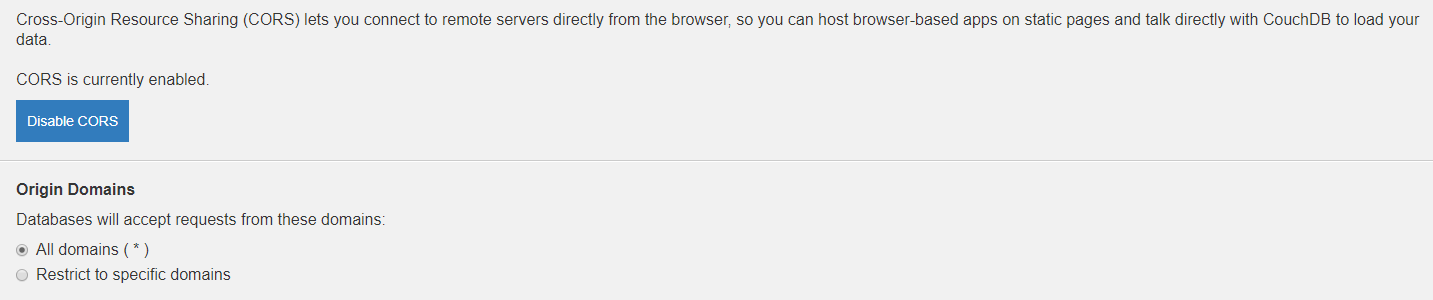
\includegraphics[width=1\linewidth]{images/CORS.PNG}
     \caption{CORS Konfiguration CouchDB}
    \label{broker}
  \end{center}
\end{figure}

